\begin{figure}[H]
    \begin{subfigure}[t]{0.5\textwidth}
        \centering
        \begin{adjustbox}{max width=0.49\textwidth}
            \centering
            % Scale factor 0.12470588235294117
\definecolor{color15}{RGB}{255,255,255}
\definecolor{color16}{RGB}{255,255,153}
\definecolor{color17}{RGB}{153,255,153}
\definecolor{color18}{RGB}{0,150,60}
\definecolor{color19}{RGB}{0,0,0}
% Bounding Box: 235.0, 170.0
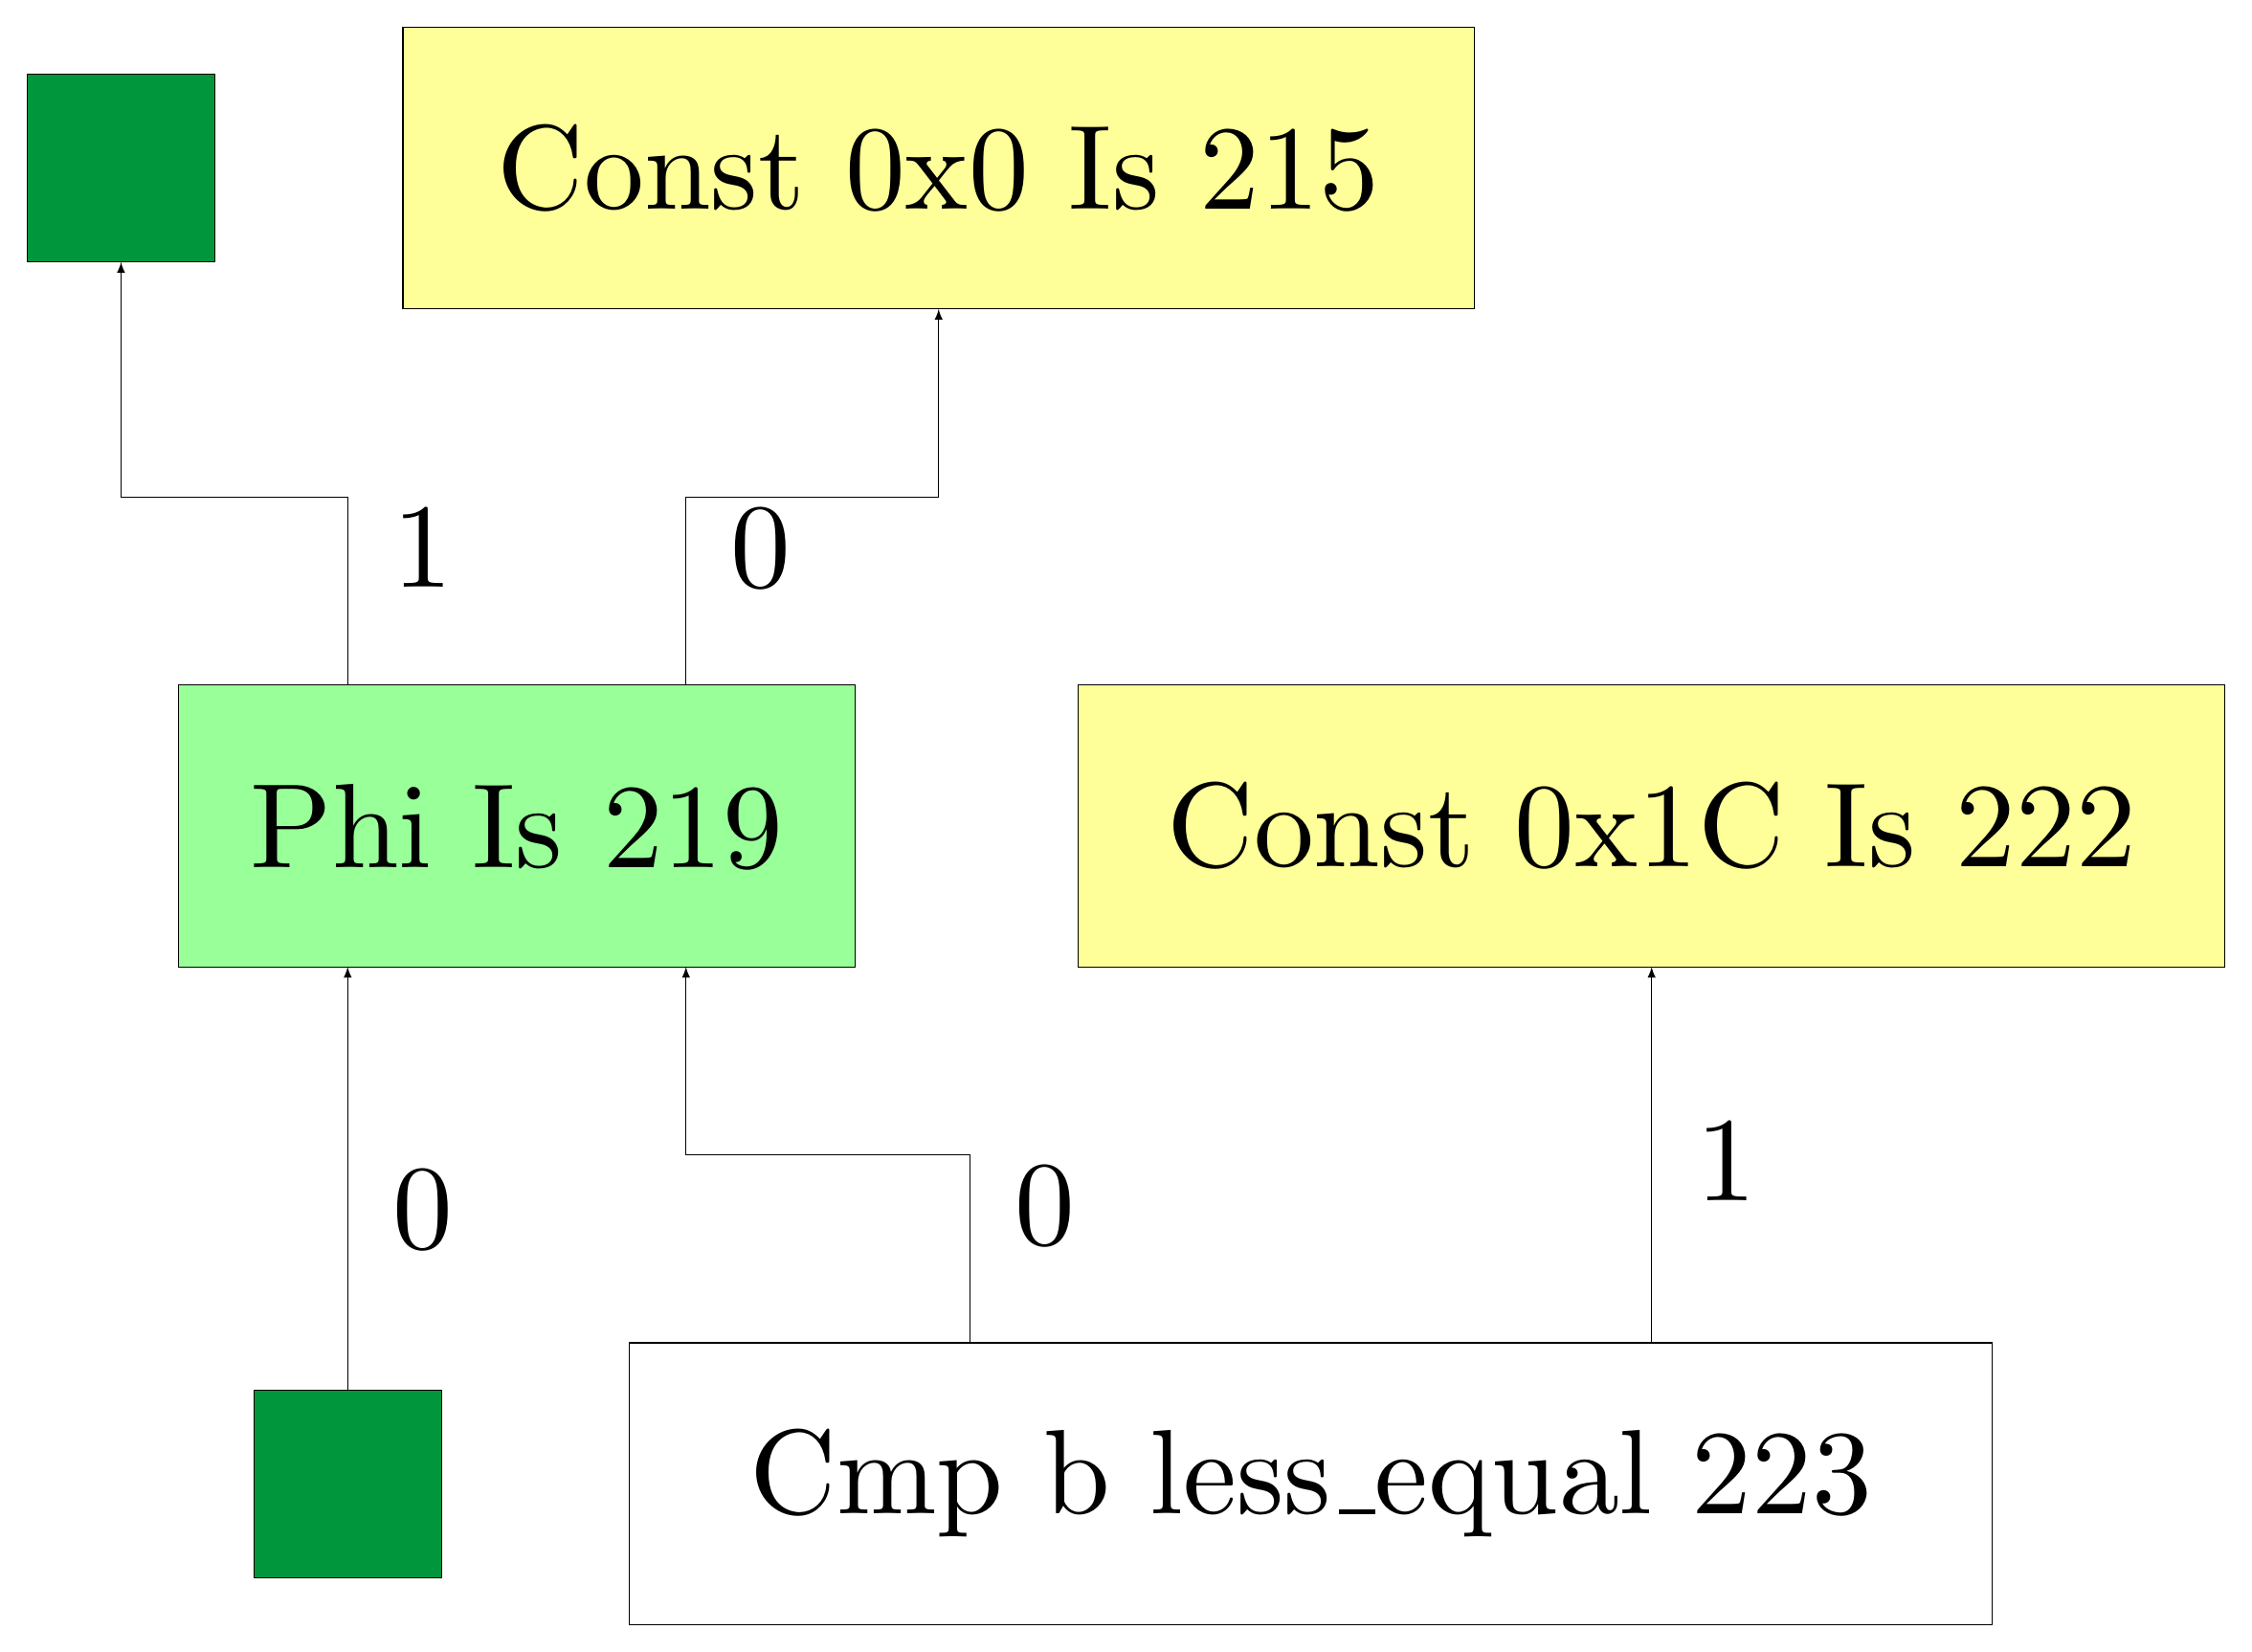
\begin{tikzpicture}
	\node[fill=color15, draw, minimum width=18.08235294117647cm, minimum height=3.741176470588235cm] (n57) at (37.13667820069204cm ,-51.37882352941176cm) {};
	% 1 node layouts
	\node[scale=4.5347593582887695, transform shape] at (37.13667820069204cm ,-51.37882352941176cm) {Cmp b less\_equal 223};
	\node[fill=color16, draw, minimum width=15.214117647058822cm, minimum height=3.741176470588235cm] (n58) at (41.65726643598616cm ,-42.64941176470588cm) {};
	% 1 node layouts
	\node[scale=4.5347593582887695, transform shape] at (41.65726643598616cm ,-42.64941176470588cm) {Const 0x1C Is 222};
	\node[fill=color17, draw, minimum width=8.978823529411764cm, minimum height=3.741176470588235cm] (n59) at (26.59903114186851cm ,-42.64941176470588cm) {};
	% 1 node layouts
	\node[scale=4.5347593582887695, transform shape] at (26.59903114186851cm ,-42.64941176470588cm) {Phi Is 219};
	\node[fill=color16, draw, minimum width=14.216470588235293cm, minimum height=3.741176470588235cm] (n60) at (32.196124567474044cm ,-33.919999999999995cm) {};
	% 1 node layouts
	\node[scale=4.5347593582887695, transform shape] at (32.196124567474044cm ,-33.919999999999995cm) {Const 0x0 Is 215};
	\node[fill=color18, draw, minimum width=2.4941176470588236cm, minimum height=2.4941176470588236cm] (n61) at (24.354325259515573cm ,-51.37882352941176cm) {};
	\node[fill=color18, draw, minimum width=2.4941176470588236cm, minimum height=2.4941176470588236cm] (n62) at (21.346712802768167cm ,-33.919999999999995cm) {};
	\draw[color=color19, -latex] (32.616089965397926cm ,-49.50823529411764cm) -- (32.616089965397926cm ,-47.01411764705882cm) -- (28.843737024221454cm ,-47.01411764705882cm) -- (28.843737024221454cm ,-44.519999999999996cm);
	\node[] at (33.61373702422145cm ,-47.69220588235294cm) {
		\scalebox{4.5347593582887695}{0}
	};
	\draw[color=color19, -latex] (41.65726643598616cm ,-49.50823529411764cm) -- (41.65726643598616cm ,-44.519999999999996cm);
	\node[] at (42.65491349480969cm ,-47.114954044117646cm) {
		\scalebox{4.5347593582887695}{1}
	};
	\draw[color=color19, -latex] (28.843737024221454cm ,-40.77882352941176cm) -- (28.843737024221454cm ,-38.28470588235294cm) -- (32.196124567474044cm ,-38.28470588235294cm) -- (32.196124567474044cm ,-35.790588235294116cm);
	\node[] at (29.841384083044982cm ,-38.96279411764706cm) {
		\scalebox{4.5347593582887695}{0}
	};
	\draw[color=color19, -latex] (24.354325259515573cm ,-40.77882352941176cm) -- (24.354325259515573cm ,-38.28470588235294cm) -- (21.346712802768167cm ,-38.28470588235294cm) -- (21.346712802768167cm ,-35.16705882352941cm);
	\node[] at (25.3519723183391cm ,-38.96279411764706cm) {
		\scalebox{4.5347593582887695}{1}
	};
	\draw[color=color19, -latex] (24.354325259515573cm ,-50.13176470588235cm) -- (24.354325259515573cm ,-44.519999999999996cm);
	\node[] at (25.3519723183391cm ,-47.738483455882346cm) {
		\scalebox{4.5347593582887695}{0}
	};
\end{tikzpicture}

        \end{adjustbox}
        \caption{The original condition with bound $N$}
    \end{subfigure}
    \begin{subfigure}[t]{0.5\textwidth}
        \centering
        \begin{adjustbox}{max width=0.49\textwidth}
            \centering
            % Scale factor 0.06838709677419355
\definecolor{color10}{RGB}{255,255,255}
\definecolor{color11}{RGB}{153,255,153}
\definecolor{color12}{RGB}{255,255,153}
\definecolor{color13}{RGB}{0,150,60}
\definecolor{color14}{RGB}{0,0,0}
% Bounding Box: 409.0, 310.0
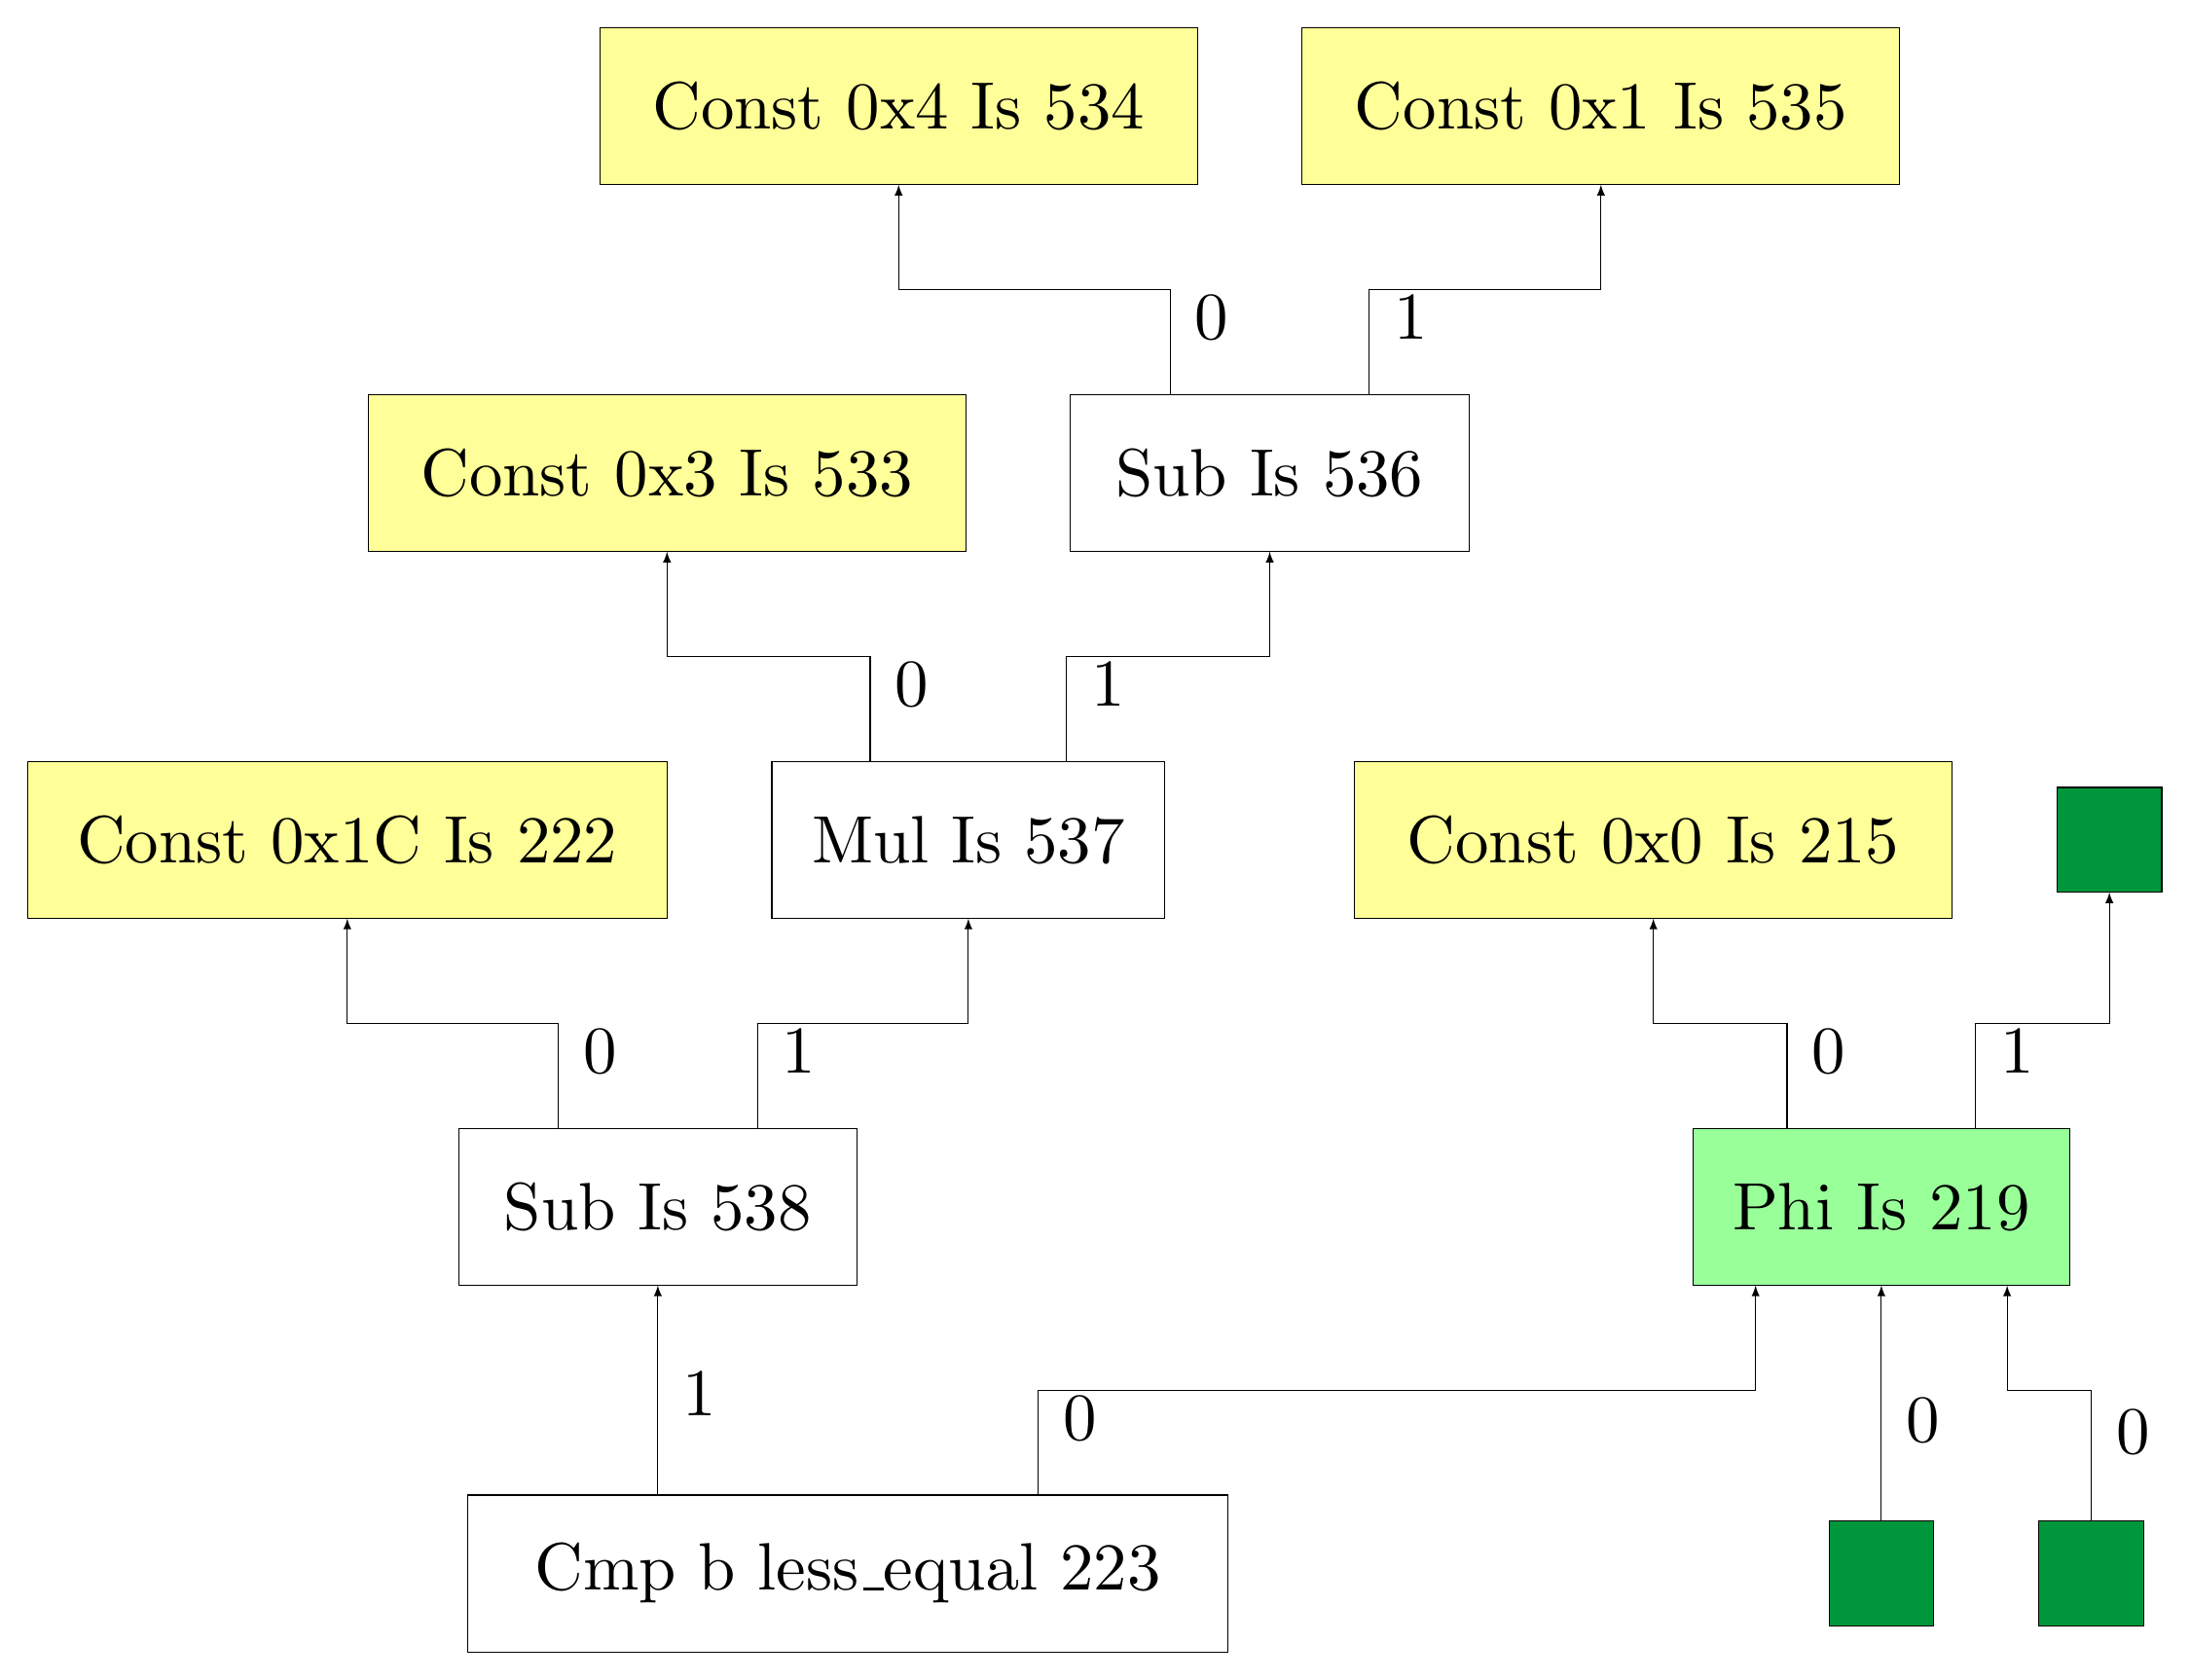
\begin{tikzpicture}
	\node[fill=color10, draw, minimum width=9.916129032258064cm, minimum height=2.0516129032258066cm] (n44) at (113.58092041890683cm ,-28.175483870967742cm) {};
	% 1 node layouts
	\node[scale=2.4868035190615836, transform shape] at (113.58092041890683cm ,-28.175483870967742cm) {Cmp b less\_equal 223};
	\node[fill=color11, draw, minimum width=4.9238709677419354cm, minimum height=2.0516129032258066cm] (n45) at (127.06635724686382cm ,-23.388387096774196cm) {};
	% 1 node layouts
	\node[scale=2.4868035190615836, transform shape] at (127.06635724686382cm ,-23.388387096774196cm) {Phi Is 219};
	\node[fill=color12, draw, minimum width=7.796129032258065cm, minimum height=2.0516129032258066cm] (n46) at (124.09151853718639cm ,-18.601290322580645cm) {};
	% 1 node layouts
	\node[scale=2.4868035190615836, transform shape] at (124.09151853718639cm ,-18.601290322580645cm) {Const 0x0 Is 215};
	\node[fill=color10, draw, minimum width=5.1974193548387095cm, minimum height=2.0516129032258066cm] (n47) at (111.10188816084231cm ,-23.388387096774196cm) {};
	% 1 node layouts
	\node[scale=2.4868035190615836, transform shape] at (111.10188816084231cm ,-23.388387096774196cm) {Sub Is 538};
	\node[fill=color12, draw, minimum width=8.343225806451613cm, minimum height=2.0516129032258066cm] (n48) at (107.04995267697134cm ,-18.601290322580645cm) {};
	% 1 node layouts
	\node[scale=2.4868035190615836, transform shape] at (107.04995267697134cm ,-18.601290322580645cm) {Const 0x1C Is 222};
	\node[fill=color10, draw, minimum width=5.129032258064516cm, minimum height=2.0516129032258066cm] (n49) at (115.15382364471328cm ,-18.601290322580645cm) {};
	% 1 node layouts
	\node[scale=2.4868035190615836, transform shape] at (115.15382364471328cm ,-18.601290322580645cm) {Mul Is 537};
	\node[fill=color12, draw, minimum width=7.796129032258065cm, minimum height=2.0516129032258066cm] (n50) at (111.22156558019715cm ,-13.814193548387097cm) {};
	% 1 node layouts
	\node[scale=2.4868035190615836, transform shape] at (111.22156558019715cm ,-13.814193548387097cm) {Const 0x3 Is 533};
	\node[fill=color10, draw, minimum width=5.1974193548387095cm, minimum height=2.0516129032258066cm] (n51) at (119.0860817092294cm ,-13.814193548387097cm) {};
	% 1 node layouts
	\node[scale=2.4868035190615836, transform shape] at (119.0860817092294cm ,-13.814193548387097cm) {Sub Is 536};
	\node[fill=color12, draw, minimum width=7.796129032258065cm, minimum height=2.0516129032258066cm] (n52) at (114.24377660170252cm ,-9.027096774193549cm) {};
	% 1 node layouts
	\node[scale=2.4868035190615836, transform shape] at (114.24377660170252cm ,-9.027096774193549cm) {Const 0x4 Is 534};
	\node[fill=color12, draw, minimum width=7.796129032258065cm, minimum height=2.0516129032258066cm] (n53) at (123.40764756944445cm ,-9.027096774193549cm) {};
	% 1 node layouts
	\node[scale=2.4868035190615836, transform shape] at (123.40764756944445cm ,-9.027096774193549cm) {Const 0x1 Is 535};
	\node[fill=color13, draw, minimum width=1.367741935483871cm, minimum height=1.367741935483871cm] (n54) at (129.80184111783154cm ,-28.175483870967742cm) {};
	\node[fill=color13, draw, minimum width=1.367741935483871cm, minimum height=1.367741935483871cm] (n55) at (130.04119595654123cm ,-18.601290322580645cm) {};
	\node[fill=color13, draw, minimum width=1.367741935483871cm, minimum height=1.367741935483871cm] (n56) at (127.06635724686382cm ,-28.175483870967742cm) {};
	\draw[color=color14, -latex] (116.05995267697135cm ,-27.14967741935484cm) -- (116.05995267697135cm ,-25.781935483870967cm) -- (125.42506692428317cm ,-25.781935483870967cm) -- (125.42506692428317cm ,-24.414193548387097cm);
	\node[] at (116.6070494511649cm ,-26.153790322580647cm) {
		\scalebox{2.4868035190615836}{0}
	};
	\draw[color=color14, -latex] (111.10188816084231cm ,-27.14967741935484cm) -- (111.10188816084231cm ,-24.414193548387097cm);
	\node[] at (111.64898493503586cm ,-25.837232862903228cm) {
		\scalebox{2.4868035190615836}{1}
	};
	\draw[color=color14, -latex] (125.83538950492833cm ,-22.36258064516129cm) -- (125.83538950492833cm ,-20.99483870967742cm) -- (124.09151853718639cm ,-20.99483870967742cm) -- (124.09151853718639cm ,-19.62709677419355cm);
	\node[] at (126.38248627912188cm ,-21.366693548387097cm) {
		\scalebox{2.4868035190615836}{0}
	};
	\draw[color=color14, -latex] (128.2973249887993cm ,-22.36258064516129cm) -- (128.2973249887993cm ,-20.99483870967742cm) -- (130.04119595654123cm ,-20.99483870967742cm) -- (130.04119595654123cm ,-19.28516129032258cm);
	\node[] at (128.84442176299285cm ,-21.366693548387097cm) {
		\scalebox{2.4868035190615836}{1}
	};
	\draw[color=color14, -latex] (109.80253332213263cm ,-22.36258064516129cm) -- (109.80253332213263cm ,-20.99483870967742cm) -- (107.04995267697134cm ,-20.99483870967742cm) -- (107.04995267697134cm ,-19.62709677419355cm);
	\node[] at (110.34963009632618cm ,-21.366693548387097cm) {
		\scalebox{2.4868035190615836}{0}
	};
	\draw[color=color14, -latex] (112.40124299955198cm ,-22.36258064516129cm) -- (112.40124299955198cm ,-20.99483870967742cm) -- (115.15382364471328cm ,-20.99483870967742cm) -- (115.15382364471328cm ,-19.62709677419355cm);
	\node[] at (112.94833977374553cm ,-21.366693548387097cm) {
		\scalebox{2.4868035190615836}{1}
	};
	\draw[color=color14, -latex] (113.87156558019714cm ,-17.575483870967744cm) -- (113.87156558019714cm ,-16.20774193548387cm) -- (111.22156558019715cm ,-16.20774193548387cm) -- (111.22156558019715cm ,-14.84cm);
	\node[] at (114.41866235439069cm ,-16.57959677419355cm) {
		\scalebox{2.4868035190615836}{0}
	};
	\draw[color=color14, -latex] (116.43608170922941cm ,-17.575483870967744cm) -- (116.43608170922941cm ,-16.20774193548387cm) -- (119.0860817092294cm ,-16.20774193548387cm) -- (119.0860817092294cm ,-14.84cm);
	\node[] at (116.98317848342296cm ,-16.57959677419355cm) {
		\scalebox{2.4868035190615836}{1}
	};
	\draw[color=color14, -latex] (117.78672687051973cm ,-12.788387096774194cm) -- (117.78672687051973cm ,-11.420645161290324cm) -- (114.24377660170252cm ,-11.420645161290324cm) -- (114.24377660170252cm ,-10.052903225806451cm);
	\node[] at (118.33382364471328cm ,-11.7925cm) {
		\scalebox{2.4868035190615836}{0}
	};
	\draw[color=color14, -latex] (120.38543654793908cm ,-12.788387096774194cm) -- (120.38543654793908cm ,-11.420645161290324cm) -- (123.40764756944445cm ,-11.420645161290324cm) -- (123.40764756944445cm ,-10.052903225806451cm);
	\node[] at (120.93253332213263cm ,-11.7925cm) {
		\scalebox{2.4868035190615836}{1}
	};
	\draw[color=color14, -latex] (129.80184111783154cm ,-27.491612903225807cm) -- (129.80184111783154cm ,-25.781935483870967cm) -- (128.70764756944445cm ,-25.781935483870967cm) -- (128.70764756944445cm ,-24.414193548387097cm);
	\node[] at (130.3489378920251cm ,-26.32475806451613cm) {
		\scalebox{2.4868035190615836}{0}
	};
	\draw[color=color14, -latex] (127.06635724686382cm ,-27.491612903225807cm) -- (127.06635724686382cm ,-24.414193548387097cm);
	\node[] at (127.61345402105736cm ,-26.179168346774194cm) {
		\scalebox{2.4868035190615836}{0}
	};
\end{tikzpicture}

        \end{adjustbox}
        \caption{The changed condition with bound $\hat{N}$}
    \end{subfigure}
    \caption{
    The change of header condition for \Cref{fig:impl:fixup:fixup-firm-loop}.
    Please note that through an implicit optimization by \libFIRM{}, the comparison has been changed to $\leq$ and hence $N$ to 28.
    }
    \label{fig:impl:fixup:header-cond:firm}
\end{figure}